\chapter{How to Run}
\label{ap: appendixB}

This appendix describes the few steps that are required to get the software running on the user's Linux machine.

\section{Running the Python GUI}
In the top level directory of the project, there should be a file titled \texttt{GUI.py} which will act as the main entry point into the project. To run this file, it can be run either as an executable with
\begin{verbatim}
    ./GUI.py
\end{verbatim}
or as a Python script with
\begin{verbatim}
    python3 GUI.py
\end{verbatim}
The output GUI is shown in Figure~\ref{fig:desktopGUI}
\begin{figure}[H]
    \centering
    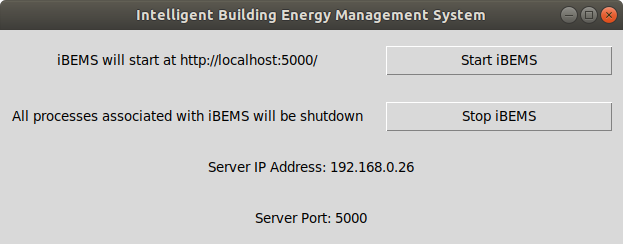
\includegraphics[scale=0.5]{figs/desktopGUI.png}
    \caption{Desktop GUI}
    \label{fig:desktopGUI}
\end{figure}

\section{Running the software}
By clicking on the "Start iBEMS" button shown in Figure~\ref{fig:desktopGUI}, the software will be launched in a new terminal shown in Figure~\ref{fig:runningterminal}.
\begin{figure}[H]
    \centering
    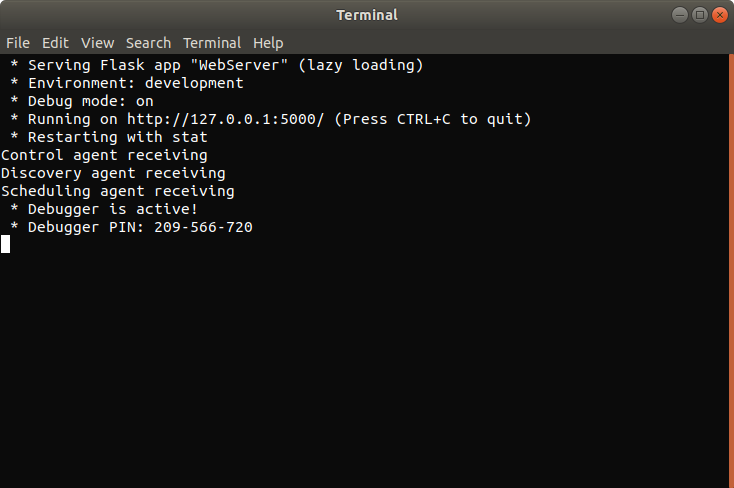
\includegraphics[scale=0.4]{figs/runningterminal.png}
    \caption{Running terminal}
    \label{fig:runningterminal}
\end{figure}
